\begin{figure*}[t]
\begin{minipage}[c]{3.33in}
  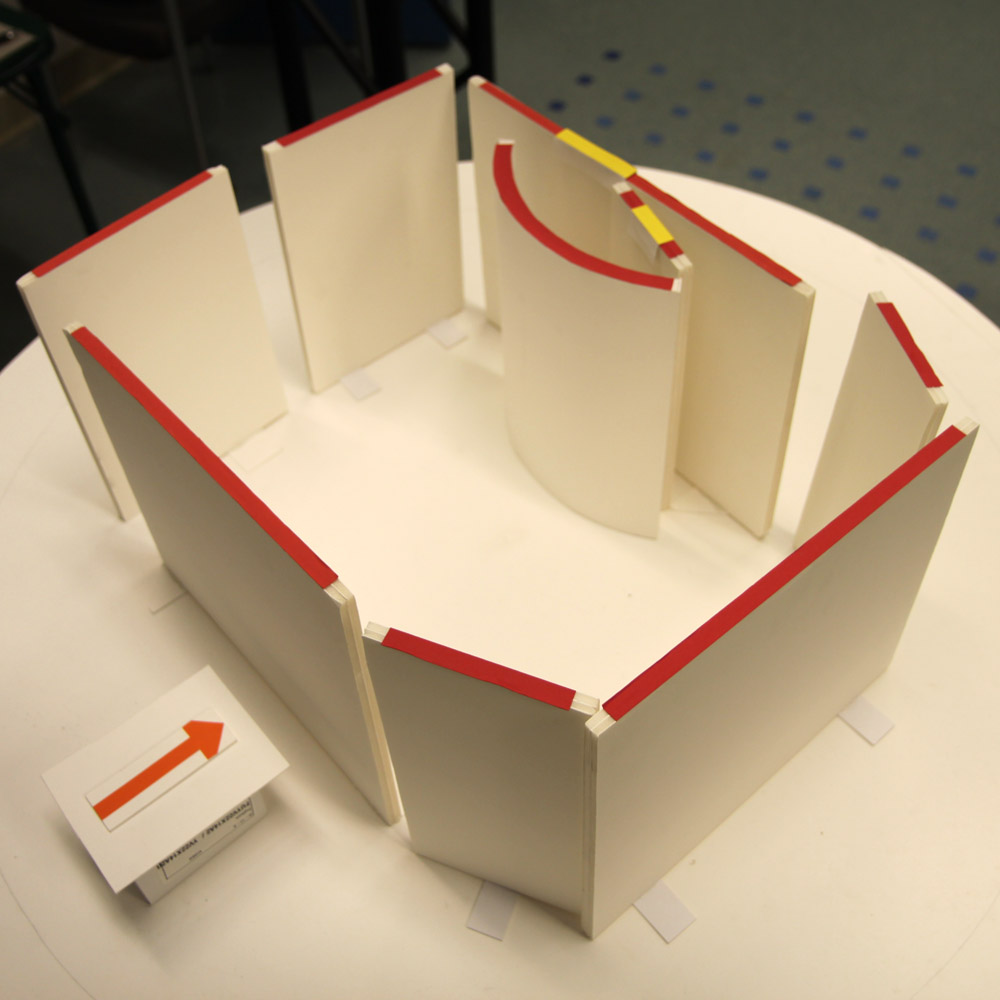
\includegraphics[width=1.65in]{../gi2012_userstudy/images/photos/38_renovation} %A2
  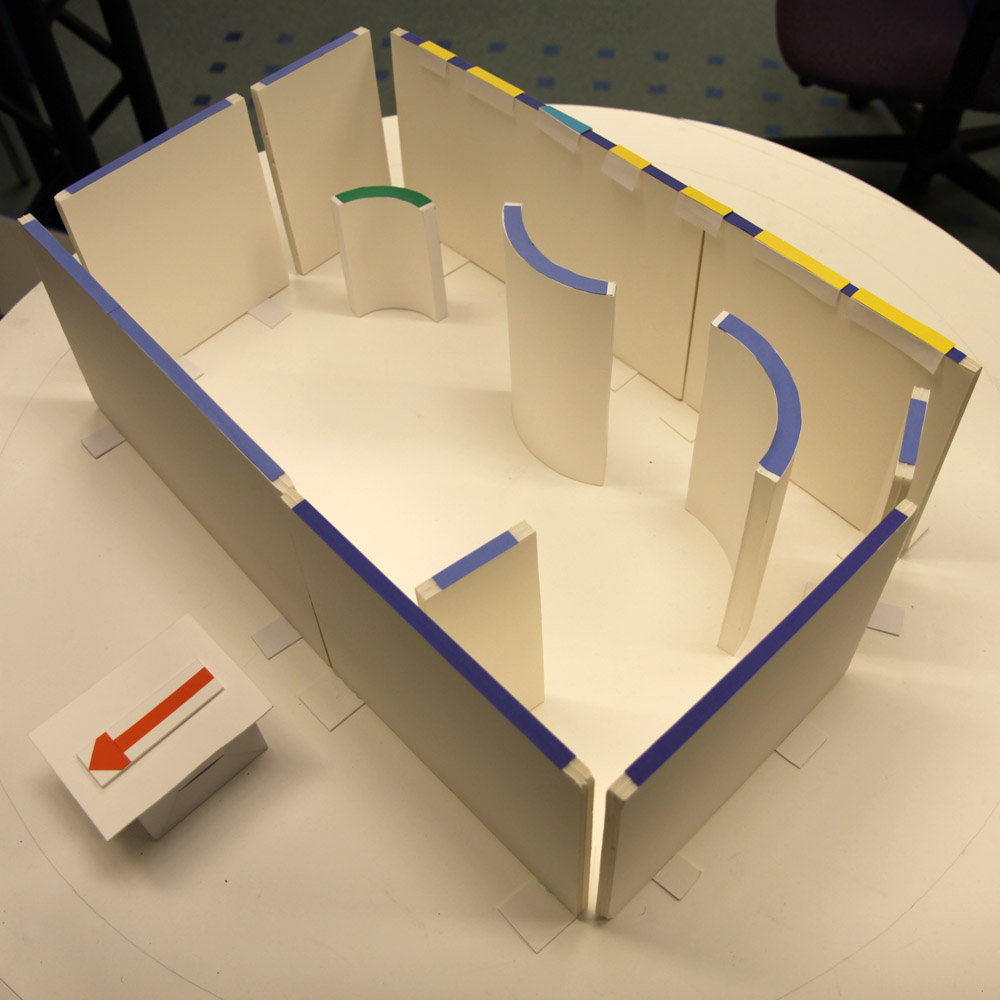
\includegraphics[width=1.65in]{../gi2012_userstudy/images/photos/42_renovation} %A3
\end{minipage}
\begin{minipage}[c]{4.9in}

  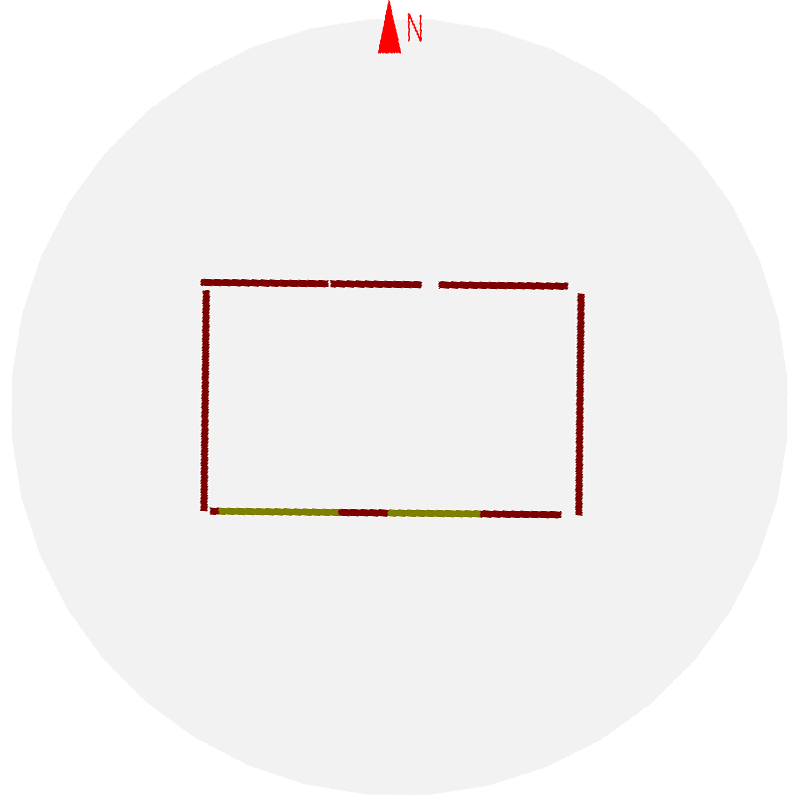
\includegraphics[width=0.9in]{../gi2012_userstudy/images/section3/0_2D_walls_rotate_edit} %A1
  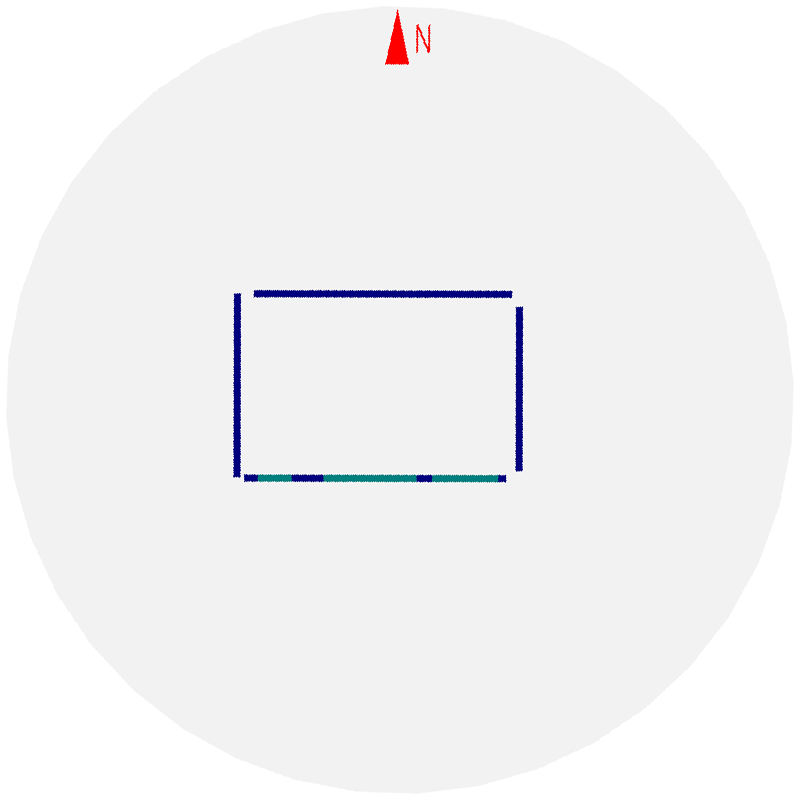
\includegraphics[width=0.9in]{../gi2012_userstudy/images/section3/6_2D_walls_rotate} %A4
  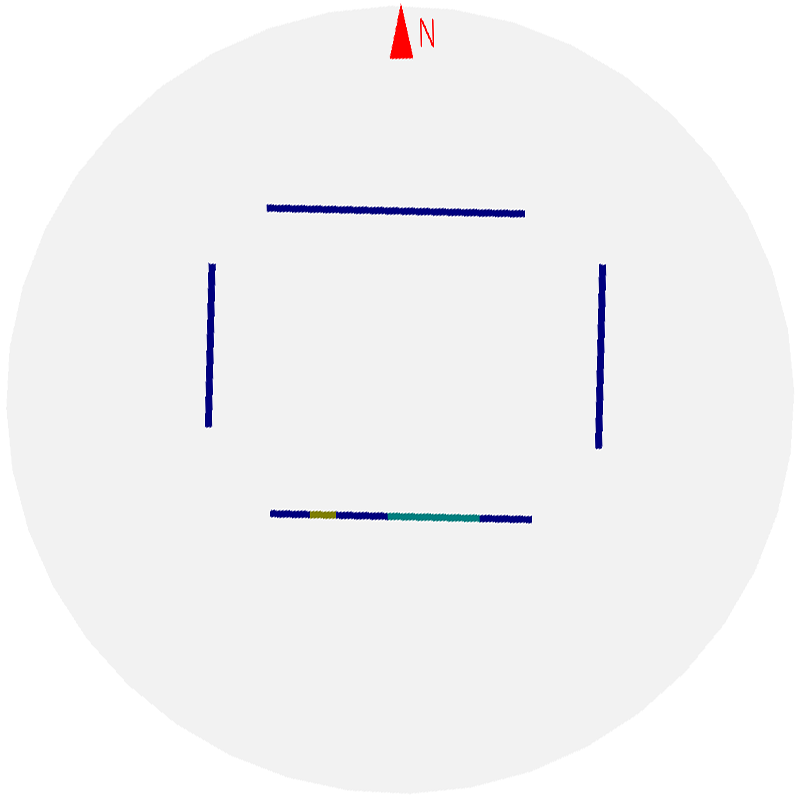
\includegraphics[width=0.9in]{../gi2012_userstudy/images/section3/7_2D_walls_rotate} %A5
  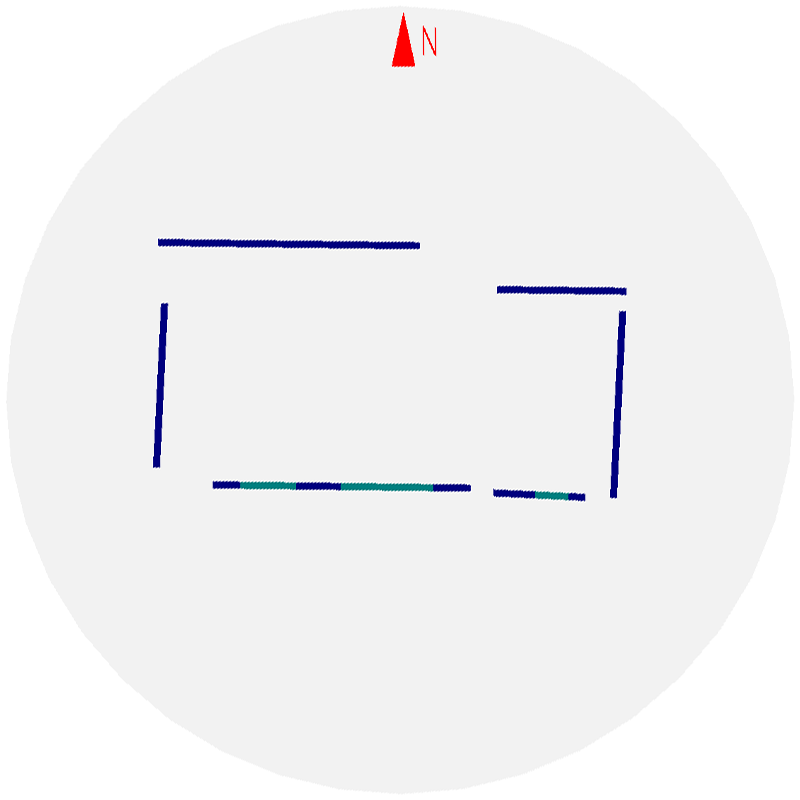
\includegraphics[width=0.9in]{../gi2012_userstudy/images/section3/8_2D_walls_rotate}\\ %A6
  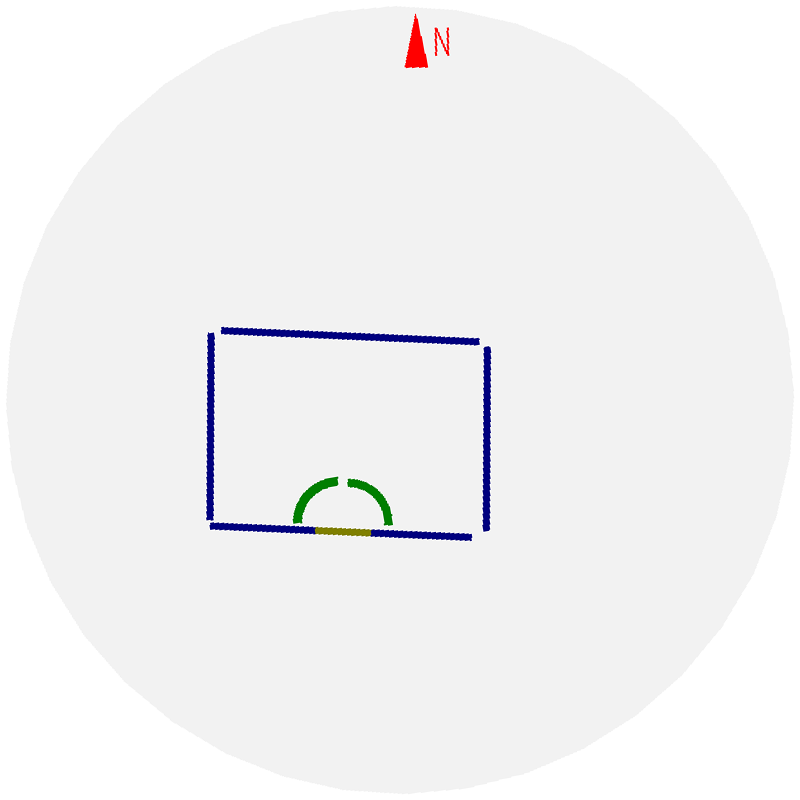
\includegraphics[width=0.9in]{../gi2012_userstudy/images/section3/2_2D_walls_rotate} %N2
  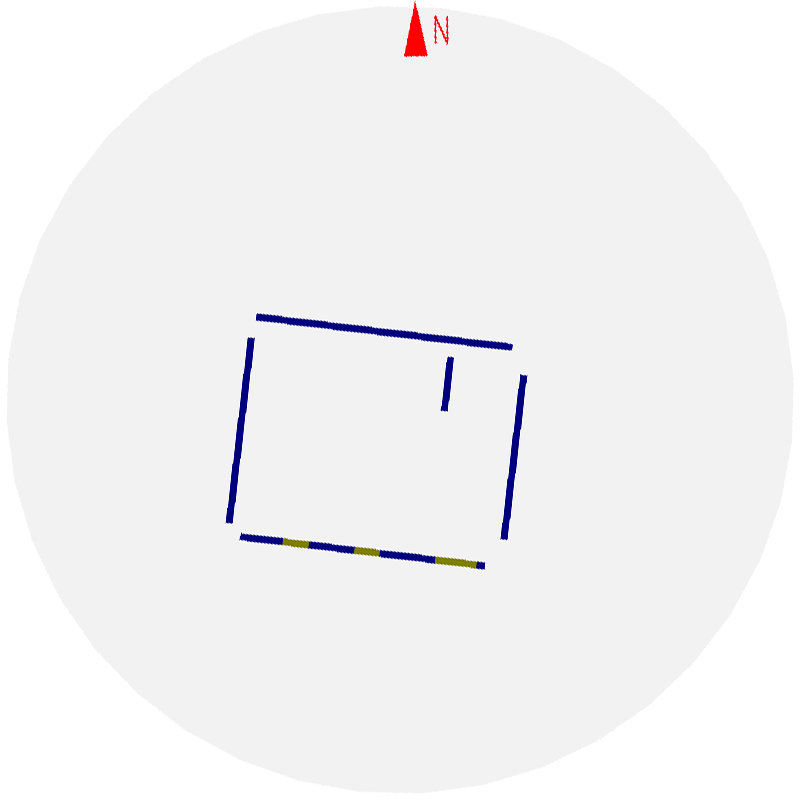
\includegraphics[width=0.9in]{../gi2012_userstudy/images/section3/3_2D_walls_rotate} %N3
  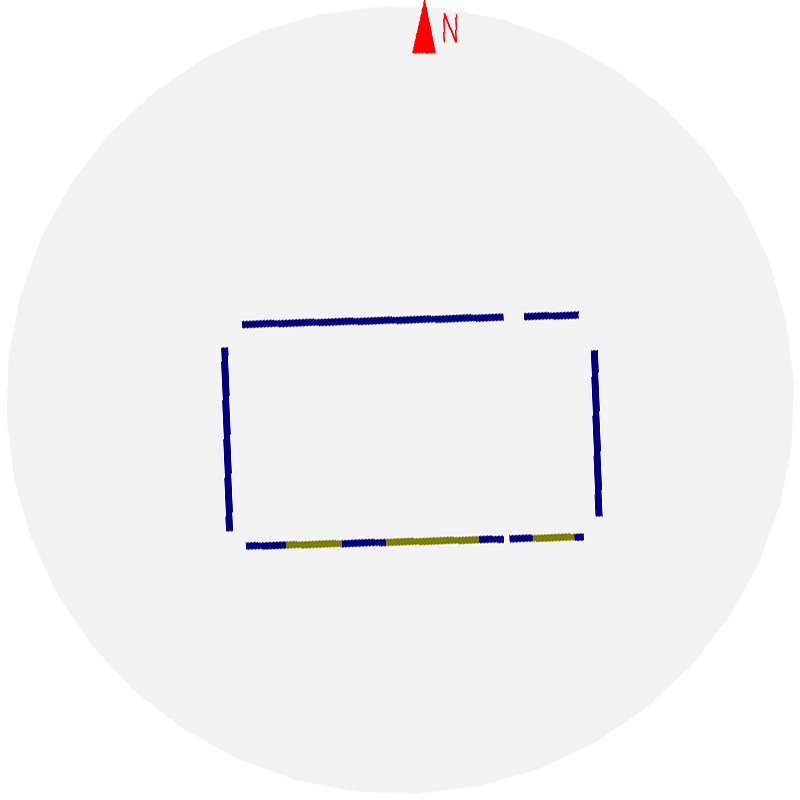
\includegraphics[width=0.9in]{../gi2012_userstudy/images/section3/4_2D_walls_rotate} %N4
  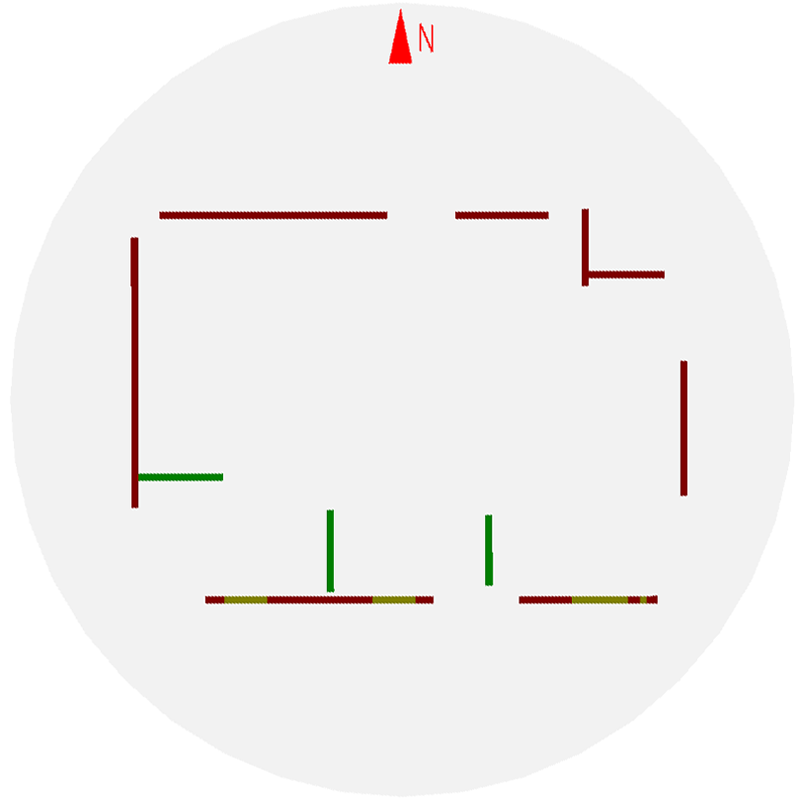
\includegraphics[width=0.9in]{../gi2012_userstudy/images/section3/9_2D_walls_rotate} %N6
\end{minipage}
\vspace{-1.12in}
\\
\begin{minipage}{1.65in}~\end{minipage}
\begin{minipage}{1.65in}~\end{minipage}
\begin{minipage}{0.9in}{\bf A1}\end{minipage}
\begin{minipage}{0.9in}{\bf A4}\end{minipage}
\begin{minipage}{0.88in}{\bf A5}\end{minipage}
\begin{minipage}{0.88in}{\bf A6}\end{minipage}%
\vspace{0.68in}
\\
\begin{minipage}{1.65in}{\bf ~A2}\end{minipage}
\begin{minipage}{1.65in}{\bf ~A3}\end{minipage}
\begin{minipage}{0.9in}{\bf N2}\end{minipage}
\begin{minipage}{0.9in}{\bf N3}\end{minipage}
\begin{minipage}{0.88in}{\bf N4}\end{minipage}
\begin{minipage}{0.88in}{\bf N6}\end{minipage}\vspace{0.0in}%
  \caption{ In Part 3 of the study participants were asked to propose
    a modest renovation to the geometry to improve the use of
    daylighting.
%Three users came up with especially creative ways to deal with glare in the space.
Renderings of several of these geometries are shown
in
Figures~\ref{figure:renovations}.
%Figures~\ref{figure:brighter_renovations}~and~\ref{figure:diffusing_renovations}.
  }
\label{figure:improved_designs}
\vspace{-0.1in}
\end{figure*}
